\chapter{General discussion}
\label{chap9}
\minitoc

\section{Toward a general model for shallow magmatic intrusion}
\label{sec:dynam-shall-magm-1}

\subsection{Summary}
\label{sec:summary-2}

\citet{Michaut:2011kg} originally provides a model which describes the
dynamics  of shallow  magmatic intrusions.   In particular,  depending
mainly  on the  injection  rate  and the  intrusion  depth, the  model
predicts  two   regimes  of  propagation  characterized   by  specific
morphologies and  scaling laws  for intrusion thickness  versus length
and  time.  This  model  predicts the  appropriate  geometry for  both
terrestrial  laccoliths and  large mafic  sills. However,  we show  in
Chapter \ref{chap2} that it  underestimates the absolute dimensions of
these magmatic intrusions; in  particular, it requires abnormally high
viscosity to reconcile both observations and predictions.

To get  some insights in the  effective flow viscosity, we  develop in
chapter \ref{C3-JFM}  and \ref{Heating} an  extension of the  model of
\citet{Michaut:2011kg} that  accounts for the cooling  of the current.
We show that  the coupling between the temperature field  and the flow
itself leads  to the formation of  a highly viscous region  at the tip
which slows  down the  spreading in both  regimes. The  intrusions are
predicted  to  be thicker  and  their  dimensions, especially  in  the
bending regime, are now consistent with the observations.

In Chapter  \ref{C5-chap6}, we  neglect the  cooling to  relax another
assumption of  the original model of  \citet{Michaut:2011kg}, i.e. the
constant thickness  of the  upper layer. In  particular, we  study the
effect of a crater depression located on top of the intrusion.  We show that
the lithostatic barrier imposed by the crater wall at the periphery of
the depression prevents  the spreading of the  intrusion which instead
thickens. This second model also shows predictions consistent with the
deformations observed at floor-fractured craters.

Promising  comparison between  predictions  and  observations such  as
these  should  drive a  methodical  and  rigorous improvement  of  the
mathematical model for the emplacement of shallow magmatic intrusions.
Nevertheless,  we also  show the  limit of  using field  observations,
whose  parameters  are  poorly  constrained,  to  validate  the  model
predictions.   An  alternative  approach  could  be  to  use  analogue
experiments that are  designed to produce some feature  of the natural
system at a  laboratory scale. Indeed, such  experiments could provide
useful   benchmarks  for   the   theoretical   model.   In   addition,
phenomenological observations not predicted  by the theory could guide
further investigations  toward our  understanding of  shallow magmatic
intrusions.

\subsection{What does limit the extent of magmatic intrusions?}
\label{sec:summary-2}

While  the crater  depression clearly  limits the  flow expansion  for
crater-centered intrusions,  one can  wonder about why  laccoliths and
sills stop  their propagation  in the third  bending phase  and second
gravity phase respectively. Available  data on terrestrial laccoliths,
used in combination  with the model, show  that terrestrial laccoliths
probably do  not stop  following the formation  of the  highly viscous
region  at  the  intrusion  front,  as  initially  suggested  (Section
\ref{Heating}).

Instead, a  tempting hypothesis  is that the  limited volume  of magma
initially   available    simply   limits    the   extent    of   these
intrusions. Indeed, one  may expect that the injection  rate, which is
considered constant in this model, wanes as the deep magma source gets
exhausted.   Depending on  the  local emplacement  conditions, if  the
injection rate lasts sufficiently long for the intrusion to transition
to the  gravity regime, the  intrusion solidifies  as a sill.   In the
contrary,  the  intrusion  solidifies  as a  laccolith.   The  current
thickness and  time at the  transition depends on the  composition. In
particular, the  more evolved  the magma  composition, the  larger the
transition time and the larger  the volume required for the transition
to  occur.   Together,  it  corroborates  the  predominance  in  field
observations of felsic laccoliths and mafic sills.

In  addition, in  chapter \ref{Heating},  we show  that a  significant
thermal aureole  should develop  in the wall  rocks above  the central
flow region. Apart from plastic rock deformation that might develop in
the encasing rocks,  the thermal erosion above the  feeder dyke, where
the  temperature  are  expected  to   be  maximum,  might  also  favor
subsequent dyke  propagation and limit  the size of the  intrusion. It
could  also  potentially  explain  the  nested  structure  of  several
laccolith      complexes      reported     in      the      literature
\citep{E:2015tl,Rocchi:2010dn}.

Alternatively, particularly for large  mafic sills, their arrest could
also  be  explain  by  fracturation  at the  front.   For  a  sake  of
simplicity, we  used a thin  prewetting film at  the tip to  avoid the
requirement of any boundary condition at a genuine front in the models
developed in this thesis. Nevertheless,  a necessary extension of this
work  is the  description of  a  realistic boundary  condition at  the
intrusion front which includes a proper stopping criterion.

\subsection{Rigorous treatment of the front}
\label{sec:rigor-treatm-front}

\subsubsection*{Fracturation}
\label{sec:fracturation}

A first step  would be to describe  the tip in term of  a fluid driven
fracture  instead of  the thin  prewetting  film. As  seen in  Section
\ref{C2-Toughness},  linear elastic  fracture mechanics  requires that
the  mode $I$  intensity factor  $K_I$  equals a  critical value,  the
fracture toughness  of the wall  rock $K_{c}$, for the  propagation to
occur. This  condition is usually  expressed in term of  an asymptotic
condition    on    the    crack     opening    $h(r,t)$    at    $r=R$
\citep{Savitski:2002gy,Bunger:2005em,Bunger:2007vs,Detournay:2014fk}.

In  such  problem,  the  thickness  equation  is  thus  coupled  to  a
description  of  the fracture  opening  based  on the  linear  elastic
fracture mechanics. \citet{Bunger:2011cb} used  this approach to solve
the  problem  of  isoviscous  shallow magmatic  intrusions  and  found
similar  results  than  \citet{Michaut:2011kg}.   Interestingly,  they
needed values for the fracture toughness  $K_c$ two or three orders of
magnitudes  larger  than  laboratory  measurements  to  reproduce  the
observations.   In addition,  they  found that  the apparent  fracture
toughness of  laccoliths is  much larger than  for large  mafic sills,
which they  attribute to potentially  crack blunting mechanism  at the
tip  of laccoliths.   This observation  is consistent  with the  rapid
formation  of  a highly  viscous  plug  at  the  tip of  the  magmatic
intrusion described in Chapter \ref{C3-JFM} and \ref{Heating}.

Nevertheless, this model also falls short to reproduce the behavior of
large  mafic sills.   In addition,  more realistic  model should  also
consider the process zone, i.e. the region of plastic rock deformation
near       the      leading       edge      of       the      fracture
\citep{Bunger:2008cl}. Furthermore,  the large negative  pressure that
developed at the front might cause desolved gasses to exsolve from the
magma \citep{Lister:2013ia}. With the formation and the evolution of a
gap filled  with gas  at the  tip of  the current,  the fluid  and the
fracture front  do not coincide  with one another, thus  requiring the
tracking of two moving boundaries.

\subsubsection*{Fluid gap}
\label{sec:fracturation}

Along      with      the     prewetting      film      regularization,
\citet{Anonymous:QWXp_4JV} propose  a second  regularization condition
where the tip of the elastic-gravity  current consists of a lag region
filled   with    gas   at    constant   negative    pressure   (Figure
\ref{C7-Sketch}).   They show  that the  solution depends  on the  gas
pressure  in the  tip  region  in similar  fashion  that the  solution
depends  on  the prewetting  film  thickness  in Chapter  \ref{chap2},
\ref{C3-JFM} and \ref{Heating}.
\begin{figure}[h!]
  \begin{center}
    \graphicspath{ {/Users/thorey/Documents/These/Manuscript/Figure/Chapter7/} }
    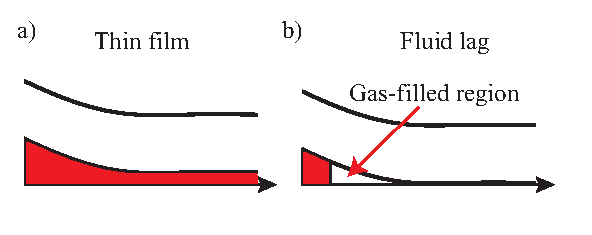
\includegraphics[scale=1.3]{Sketch.eps}
    \caption{Two different  regularization condition  at the  front of
      the current: a) thin prewetting film with thickness $h_f$ b) gas
      -filled region.}
    \label{C7-Sketch}
  \end{center}
\end{figure}
In particular, in a Cartesian geometry, they show that
\begin{eqnarray}
  h_0&\propto& h_f^{-1/7}\nu^{-2/7}L^{10/7}~(\text{Thin film})\\
  h_0&\propto& \sigma^{1/9}\nu^{-2/9}L^{14/9}~(\text{Fluid lag})
\end{eqnarray}
where $L$  is the half  length of the  flow, $-\sigma$ is  the contant
negative  pressure  in  the  fluid   lag  and  we  have  rescaled  the
characteristic    thickness    and     time    by    $\nu^{1/4}$    in
\citet{Anonymous:QWXp_4JV}.    As   expected,    the   two   different
regularization conditions lead  to only minor change  in the thickness
to length relationship ($10/7\sim 1.4$, $14/9\sim 1.5 $).

A rigorous  treatment of the front  can thus be taken  to provide only
higher-order corrections to the leading order behavior captured by the
models developed in this  thesis. Nevertheless, a complete description
of the dynamics  of the cooling gas-filled region,  where the pressure
is not  a parameter  but self consistently  determined, along  with an
appropriate fracture  condition at the  tip would surely  complete the
description provides in this thesis.


\subsection{Further model improvement}
\label{sec:generalization-model}

\subsubsection*{Heat budget}
\label{subsubsection}

The theoretical  model for the cooling  elastic-plated gravity current
assumes that the initial temperature of  the wall rock is equal to the
temperature of  the magma solidus,  i.e. $\approx 700 \celsius$  for a
felsic composition and  $\approx 1000 \celsius$ for  more mafic lavas.
However, these temperatures are large in comparison to the temperature
at the  depth of  emplacement; $\lessapprox  150 \celsius$  assuming a
geothermal gradient  of $\approx 30  \celsius$ km$^{-1}$ in  the upper
crust.   This effect  might  enhance the  cooling  and accelerate  the
transition phases in both regimes.

Viscous heating  is another mechanism  not taken into account  in this
study  that would  participate  to the  global  heat budget.   Indeed,
especially  for large  values of  $Pe$ where  we have  shown that  the
temperature   gradient  within   the   flow   are  stronger   (Section
\ref{C4-sec:infl-therm-bound-el}), the effect of viscous heating could
be important.   \citet{Costa:2005bq} have  already shown  that viscous
heating  plays  an important  role  in  the  dynamics of  fluids  with
strongly  temperature-dependent viscosity.   In  particular, for  lava
tube, they show that the heat generated by viscous friction produces a
local  temperature increase  near  the tube  walls  with a  consequent
decrease  of   the  viscosity   which  may  dramatically   change  the
temperature             and              velocity             profiles
\citep{Costa:2002cj,Costa:2003wk,Costa:2005bq}.      The     important
gradients within  the thermal  boundary layer or  near the  tip region
could  present  favorable  conditions  for  the  development  of  such
instabilities.

\subsubsection*{Stretching of the upper layer}
\label{subsubsection}

If the thickness of the intrusion  $h_0$ becomes large compared to the
intrusion depth $d_0$, the  analysis described in Chapter \ref{C3-JFM}
and  \ref{Heating}  is  not  valid  anymore. It  could  be  the  case,
especially for felsic intrusions characterized by large injection rate
intruding a layer such that $d_0\lessapprox 500$ m. In such situation,
the stretching  of the  upper layer  can no  longer be  neglected when
calculating the elastic stresses and  fluid pressure.  In that case, a
complete description  of the flow  in an axysimmetrical  and Cartesian
geometry for an isoviscous flow,  along with scaling laws for $h_0(t)$
and $R(t)$,  has already  been described by  \citet{Lister:2013ia} and
\citet{Anonymous:QWXp_4JV} respectively.  While the time dependence of
the scaling law are somewhat similar from those derived in the bending
dominated regime, the shape of the  flow is not bell-shaped anymore in
the early time solution and show a somewhat conical shape instead. For
instance, this  model could potentially  explain the conical  shape of
some     felsic      laccoliths     observed     in      Island     by
\citet{Anonymous:jHnLP36x}.
\begin{figure}[h!]
  \begin{center}
    \graphicspath{ {/Users/thorey/Documents/These/Manuscript/Figure/Chapter7/} }
    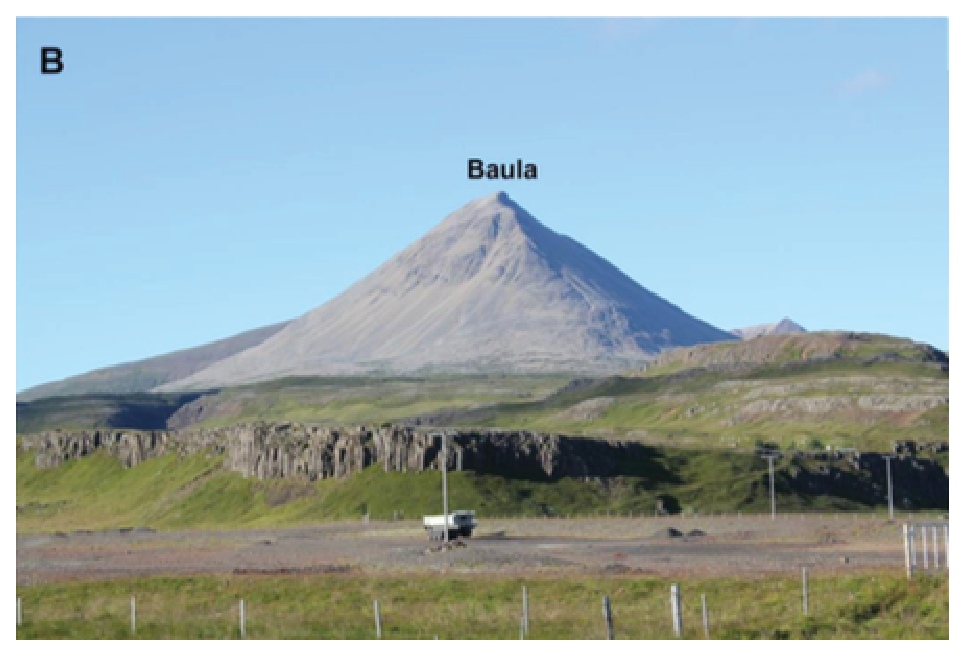
\includegraphics[scale=0.7]{Baula.eps}
    \caption{Felsic laccolith, named Baula,  in West Island.  Modified
      from \citet{Anonymous:jHnLP36x}.}
    \label{C7-Baula}
  \end{center}
\end{figure}

\subsubsection{Topography}
\label{sec:topography-1}

In Chapter \ref{C5-chap6},  we show that the topography on  top of the
intrusion can have a significant  influence on the dynamics. On Earth,
this  model could  for  instance  also be  used  to  model the  unrest
observed at volcanic calderas in  different locations across the world
\citep{Macedonio:2014et}. In addition, replacing the crater depression
by a conic volcanic edifice, the  model could also help understand the
ground deformations experienced by active volcano as a response to the
dynamics         of        underground         magmatic        systems
\citep{Cayol:2014vo,Pedersen:2004kp,Patane:2006hn,Bonaccorso:2001iw,ChadwickJr:1995cz,Cannavo:2015fk}.
In addition, the real monitoring of the deformation could also provide
benchmark for the theoretical model in this case.

\section{Lunar intrusive magmatism}
\label{sec:terr-intr-magm}

\subsection{Summary}
\label{sec:summary}

In this thesis, we focus on  two proposed candidates for shallow lunar
magmatic intrusions: low-slope domes  and floor-fractured craters.  In
Chapter \ref{Heating}, we first show  that the morphology of low-slope
lunar  domes  is  indeed   consistent  with  their  intrusive  origin.
Adapting the model of elastic-plated  gravity current model to account
for the crater depression, we then show in Chapter \ref{C5-chap6} that
the  deformations   observed  at  floor-fractured  craters  are  also
consistent  with the  emplacement of  magmatic intrusions  below their
floor.

Upon cooling and solidification,  crater-centered intrusions should be
denser than the surrounding medium and leave a positive anomaly in the
lunar gravity field.  Using the  intrusion morphology deduced from the
model, the lunar gravity field  obtained from the NASA’s GRAIL mission
and topographic  data obtained  from the LOLA  instrument, we  show in
Chapter  \ref{chap7} that  their  gravitational  signatures is  indeed
larger that the one of normal  impact craters, especially in the lunar
highlands.

Around  $10$ low-slope  lunar  domes and  about $200$  floor-fractured
craters have been detected at the  lunar surface, most of them located
close  or within  the lunar  maria. While  the total  volume of  these
magmatic intrusions should not exceed $1\%$ of the lunar maria volume,
it advocates the  presence of numerous shallow  magmatic intrusions in
the lunar crust.

\subsection{Origin of the magma}
\label{sec:crust-magm-intr}

In Chapter  \ref{C5-chap6}, we claim  that the absence  of deformation
surrounding floor-fractured craters suggests  that the unload pressure
associated with  the crater depression  might have drive  magma ascent
below these craters. However, the unload pressure, associated with the
depression, should decrease rapidly with depth on a length scale equal
to   the   crater   diameter,    i.e.    some   tens   of   kilometers
\citep{Pinel:2000wa}. Hence,  the depression caused by  the impact can
drive magma flow  if the magma is already present  on a similar length
scale,   i.e.   within   the   crust.   The   presence   of   numerous
floor-fractured craters thus raises the  question of deeper and larger
magmatic reservoirs within  the lunar crust which  might be observable
in the lunar gravity field obtained from the GRAIL mission.

This idea is also supported by recent works on rift volcanism on Earth
showing that a depression can play a crucial role in the trajectory of
magma  on the  local scale  \citep{Maccaferri:2014ft}. In  particular,
\citet{Maccaferri:2014ft} show  that the  graben depression  favor the
formation  of a  stress  barrier  at depth  which  might prevent  dyke
propagation depending  of its  nucleation depth. In  particular, dykes
nucleated deep  below the graben will  tend to be deviated  from their
vertical   trajectory  and   produce   off-rift  volcanism.    Similar
investigation in  a lunar  setting might  also demonstrate  that dykes
initiated deep within  the lunar mantle should have  been deviated off
the  crater   depression  sustaining  the  idea   of  shallower  magma
reservoir.

In the end,  a detailed analysis of the stress  field below the crater
depression  might  be the  natural  extension  of  our work  on  lunar
intrusive  magmatism;  in  particular,  it  might  explain  why  these
craters,  apart from  the underlying  low density breccia, provide  a
favorable environment for magmatic intrusions.

At a regional  scale, it could also prove fruitful  to investigate the
link  between the  load of  the lunar  maria and  the distribution  of
floor-fractured craters, which  are mainly located at the  edge of the
maria itself.
\subsection{Constraining the thickness of the lunar maria}
\label{sec:thickn-lunar-maria}

Approximately $16\%$ of the Moon's surface is covered by basaltic lava
flows  that comprise  the lunar  maria. Although  the total  extent of
these lava  flows is  known, their thicknesses  are more  difficult to
constrain \citep{Thomson:2009eo}. Many  approaches, including indirect
techniques as gravity, seismic or  radar data, or direct measurements,
through analyses of impact that  have completely penetrated the maria,
have been proposed to  estimate their thicknesses.  The elastic-plated
gravity current  models provided in  this thesis  can also be  used to
provide  estimate useful  to constrain  thickness model  of the  lunar
maria.  Indeed,  if the intrusion  has stopped in the  bending regime,
the  inequality  $R<   4\Lambda$  in  the  case  of   lunar  domes  or
$R<4\Lambda/C$ in the case of  floor-fractured craters, provide for an
estimate for  the elastic thickness  and thus,  a lower bound  for the
maria thickness

\section{Probing intrusive magmatism on other terrestrial planets}
\label{sec:other-terr-plan}

This thesis,  closely combining  theoretical models  and observations,
have  shown fruitful  in  probing the  importance  of lunar  intrusive
magmatism. In particular, the method developed in this thesis could be
carried out on other terrestrial planets. 

\citet{Michaut:2013dr}  has  already  used its  theoretical  model  to
assess the intrusive origin of several martian domes. As proven of the
Moon, floor-fractured craters are also a good first basis to probe the
importance of intrusive magmatism  on terrestrial planets.  While they
have first  been observed  and described on  the Moon,  many evidences
show now that  floor-fractured craters might be a  common landscape on
terrestrial planets.

\begin{figure}[htpb]
  \begin{center}
    \graphicspath{ {/Users/thorey/Documents/These/Manuscript/Figure/Chapter7/} }
    \includegraphics[scale=0.9]{FFCOther.eps}
    \caption{a),  b) and  c) Sample  from the  Marsian FFC  population
      located  respectively  at ($0.0^{\circ}$N,$337.3  ^{\circ}  $E),
      ($5.5^{\circ}$S,$322.6         ^{\circ}          $E)         and
      ($6.7^{\circ}$S,$333.4^{\circ}$E).   All are  TEHMIS daytime  IR
      image taken modified from  \citet{Sato:2010ex}. d) Potential FFC
      on Mercury reproduced  from \citet{Schultz:1977ec}. e) Barrymore
      crater, $50$ km diameter, located  near Imdr Regio. f) Mona lisa
      Crater,  $85$ km  in diameter,  located  on the  edge of  Eistla
      Regio.   Both  are potential  FFCs  on  Venus.  Reproduced  from
      \citet{Wichman:1995ju}.}
    \label{C7-FFCOther}
  \end{center}
\end{figure}

\begin{itemize}
\item  \textbf{Mars}: On  mars, almost  $200$ floor-fractured  craters
  have also been reported located mostly  along a narrow band south of
  the dichotomy  boundary in Arabia Terra  \citep{Bamberg:2014hb}. The
  observed deformations  within these craters  is very similar  to the
  one observed on the Moon, though Marsian floor-fracture craters tend
  to  exhibit a  more  extensive and  wider  fracture network  (Figure
  \ref{C7-FFCOther}  a,  b  and  c). This  is  attributed  to  complex
  interaction of  the magmatic  intrusion with potential  ice/water in
  the  subsurface  \citep{Sato:2010ex,Bamberg:2014hb}. In  particular,
  the  melting  of the  water  (or  possibly  CO$_2$) trapped  in  the
  subsurface  would enhance  erosion of  the floor-fractured  which is
  consistent  with   some  small  and  medium   size  fluvial  outlets
  \citep{Sato:2010ex}.

  Interestingly,  deformations on  Martian floor-fractured  craters is
  not localized within the crater wall but can also extend further the
  crater rim (Figure \ref{C7-FFCOther} b,c).  In contrast to the Moon,
  the overpressure driving  the intrusion might have  been larger than
  the unloading pressure associated  with the depression. In addition,
  Martian magma,  at the  difference of  their lunar  counterpart, are
  most  likely to  be  buoyant  until the  surface  and the  mechanism
  favorable to intrusion below Martian  crater is still debated. Again
  on  Mars,  studying the  stress  field  associated with  the  crater
  depression  could  provide  a  viable  mechanism  to  trigger  magma
  spreading at depth below these craters.

\item   \textbf{Mercury}    \citet{Schultz:1977ec}   propose   several
  candidates  searching for  intra-crater dark  haloes or  other color
  variations  indicating post-impact  emplacement  of mafic  materials
  onto the floor. They did find several crater floors with contrasting
  deposits, and additionally a few rimmed moat-like depression (Figure
  \ref{C7-FFCOther} d).

\item \textbf{Venus}: Venus geologic record  have been largely cut off
  by  resurfacing events  constantly reworking  the Venusian  surface.
  Nevertheless, several candidates have also been proposed on Venus by
  \citet{Wichman:1995ju}.
\end{itemize}

Though most of these observations,  except for Marsian FFCs, have been
made in  the late nineties, they  provide an extremely good  basis for
work using new data and new methods at hand today.

%%% Local Variables:
%%% mode: latex
%%% TeX-master: "../main"
%%% End:
